\section{Experiments and Results}
\label{sec:experiments}

% \begin{figure}[t]
%   \centering
%     % \makebox[\textwidth][c]{
%     %     % \begin{tikzpicture}
%     \tikzstyle{every node}=[font=\scriptsize]
%     \definecolor{tabblue}{RGB}{31, 119, 180}
\definecolor{taborange}{RGB}{255, 127, 14}
\definecolor{tabgreen}{RGB}{44, 160, 44}
\definecolor{tabred}{RGB}{214, 39, 40}
\definecolor{tabpurple}{RGB}{148, 103, 189}
\definecolor{tabbrown}{RGB}{140, 86, 75}
\definecolor{tabpink}{RGB}{227, 119, 194}
\definecolor{tabgray}{RGB}{127, 127, 127}
\definecolor{tabolive}{RGB}{188, 189, 34}
\definecolor{tabcyan}{RGB}{23, 190, 207}
\definecolor{ForestGreen}{RGB}{34, 139, 34}
%     \begin{axis}[%
%     hide axis,
%     xmin=10,
%     xmax=50,
%     ymin=0,
%     ymax=0.1,
%     legend style={
%         draw=white!15!black,
%         legend cell align=left,
%         legend columns=3,
%         legend style={
%             draw=none,
%             column sep=1ex,
%             line width=1pt,
%         }
%     },
%     ]

%     \addlegendimage{
%         line legend,
%         tabblue,
%         thick,
%         mark=square*,
%         mark options={line width=1.5pt, rotate=45}
%     }
%     \addlegendentry{\textbf{PEACH Encoder} (Ours)}
%     \addlegendimage{line legend, tabgreen, thick, mark=triangle*, mark options={line width=1.5pt, rotate=0}}
%     \addlegendentry{GNN Encoder}
%     \addlegendimage{
%         line legend,
%         taborange,
%         thick,
%         mark=square*,
%         mark options={line width=1.5pt, rotate=0}
%     }
%     \addlegendentry{PSTNet Encoder}
%     % New Line
%     % \addlegendimage{empty legend}
%     % \addlegendentry{}

%     \addlegendimage{line legend, tabolive, thick, mark=x, mark size=3pt, mark options={line width=1pt}}
%     \addlegendentry{Oracle Encoder}
%     \addlegendimage{line legend, tabcyan, thick, mark=+, mark size=2.5pt, mark options={line width=2pt}}
%     \addlegendentry{MaNGO Mesh Encoder}
%     \addlegendimage{line legend, tabgray, thick, mark=*}
%     \addlegendentry{No Context Encoder}    
%     \end{axis}
% \end{tikzpicture}

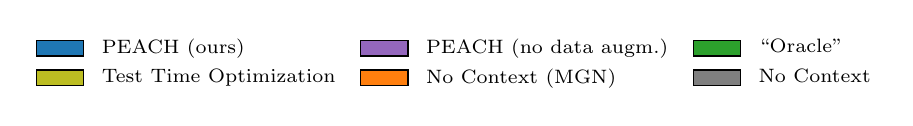
\begin{tikzpicture}
    \tikzstyle{every node}=[font=\scriptsize]
    \definecolor{tabblue}{RGB}{31, 119, 180}
\definecolor{taborange}{RGB}{255, 127, 14}
\definecolor{tabgreen}{RGB}{44, 160, 44}
\definecolor{tabred}{RGB}{214, 39, 40}
\definecolor{tabpurple}{RGB}{148, 103, 189}
\definecolor{tabbrown}{RGB}{140, 86, 75}
\definecolor{tabpink}{RGB}{227, 119, 194}
\definecolor{tabgray}{RGB}{127, 127, 127}
\definecolor{tabolive}{RGB}{188, 189, 34}
\definecolor{tabcyan}{RGB}{23, 190, 207}
\definecolor{ForestGreen}{RGB}{34, 139, 34}

    \begin{axis}[%
        hide axis,
        xmin=10,
        xmax=50,
        ymin=0,
        ymax=0.1,
        legend style={
            draw=none,
            legend cell align=left,
            legend columns=3,
            /tikz/every odd column/.append style={column sep=1ex},
            /tikz/every even column/.append style={column sep=1.6ex},
        }
    ]

    % --- Bar-style legend entries ---
    \addlegendimage{area legend, fill=tabblue}
    \addlegendentry{PEACH (ours)}

    \addlegendimage{area legend, fill=tabpurple}
    \addlegendentry{PEACH (no data augm.)}

    \addlegendimage{area legend, fill=tabgreen}
    \addlegendentry{``Oracle''}


    \addlegendimage{area legend, fill=tabolive}
    \addlegendentry{Test Time Optimization}

    
    \addlegendimage{area legend, fill=taborange}
    \addlegendentry{No Context (MGN)}

    \addlegendimage{area legend, fill=tabgray}
    \addlegendentry{No Context}
    \end{axis}
\end{tikzpicture}
%     % }
%     \makebox[\textwidth][r]{%
%   \makebox[0.77\textwidth][c]{%
%     % \begin{tikzpicture}
%     \tikzstyle{every node}=[font=\scriptsize]
%     \definecolor{tabblue}{RGB}{31, 119, 180}
\definecolor{taborange}{RGB}{255, 127, 14}
\definecolor{tabgreen}{RGB}{44, 160, 44}
\definecolor{tabred}{RGB}{214, 39, 40}
\definecolor{tabpurple}{RGB}{148, 103, 189}
\definecolor{tabbrown}{RGB}{140, 86, 75}
\definecolor{tabpink}{RGB}{227, 119, 194}
\definecolor{tabgray}{RGB}{127, 127, 127}
\definecolor{tabolive}{RGB}{188, 189, 34}
\definecolor{tabcyan}{RGB}{23, 190, 207}
\definecolor{ForestGreen}{RGB}{34, 139, 34}
%     \begin{axis}[%
%     hide axis,
%     xmin=10,
%     xmax=50,
%     ymin=0,
%     ymax=0.1,
%     legend style={
%         draw=white!15!black,
%         legend cell align=left,
%         legend columns=3,
%         legend style={
%             draw=none,
%             column sep=1ex,
%             line width=1pt,
%         }
%     },
%     ]

%     \addlegendimage{
%         line legend,
%         tabblue,
%         thick,
%         mark=square*,
%         mark options={line width=1.5pt, rotate=45}
%     }
%     \addlegendentry{\textbf{PEACH Encoder} (Ours)}
%     \addlegendimage{line legend, tabgreen, thick, mark=triangle*, mark options={line width=1.5pt, rotate=0}}
%     \addlegendentry{GNN Encoder}
%     \addlegendimage{
%         line legend,
%         taborange,
%         thick,
%         mark=square*,
%         mark options={line width=1.5pt, rotate=0}
%     }
%     \addlegendentry{PSTNet Encoder}
%     % New Line
%     % \addlegendimage{empty legend}
%     % \addlegendentry{}

%     \addlegendimage{line legend, tabolive, thick, mark=x, mark size=3pt, mark options={line width=1pt}}
%     \addlegendentry{Oracle Encoder}
%     \addlegendimage{line legend, tabcyan, thick, mark=+, mark size=2.5pt, mark options={line width=2pt}}
%     \addlegendentry{MaNGO Mesh Encoder}
%     \addlegendimage{line legend, tabgray, thick, mark=*}
%     \addlegendentry{No Context Encoder}    
%     \end{axis}
% \end{tikzpicture}

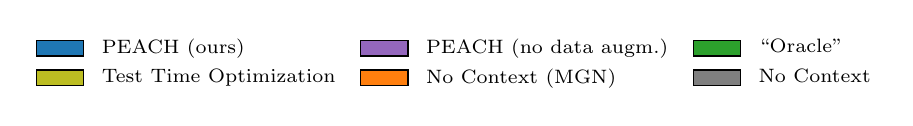
\begin{tikzpicture}
    \tikzstyle{every node}=[font=\scriptsize]
    \definecolor{tabblue}{RGB}{31, 119, 180}
\definecolor{taborange}{RGB}{255, 127, 14}
\definecolor{tabgreen}{RGB}{44, 160, 44}
\definecolor{tabred}{RGB}{214, 39, 40}
\definecolor{tabpurple}{RGB}{148, 103, 189}
\definecolor{tabbrown}{RGB}{140, 86, 75}
\definecolor{tabpink}{RGB}{227, 119, 194}
\definecolor{tabgray}{RGB}{127, 127, 127}
\definecolor{tabolive}{RGB}{188, 189, 34}
\definecolor{tabcyan}{RGB}{23, 190, 207}
\definecolor{ForestGreen}{RGB}{34, 139, 34}

    \begin{axis}[%
        hide axis,
        xmin=10,
        xmax=50,
        ymin=0,
        ymax=0.1,
        legend style={
            draw=none,
            legend cell align=left,
            legend columns=3,
            /tikz/every odd column/.append style={column sep=1ex},
            /tikz/every even column/.append style={column sep=1.6ex},
        }
    ]

    % --- Bar-style legend entries ---
    \addlegendimage{area legend, fill=tabblue}
    \addlegendentry{PEACH (ours)}

    \addlegendimage{area legend, fill=tabpurple}
    \addlegendentry{PEACH (no data augm.)}

    \addlegendimage{area legend, fill=tabgreen}
    \addlegendentry{``Oracle''}


    \addlegendimage{area legend, fill=tabolive}
    \addlegendentry{Test Time Optimization}

    
    \addlegendimage{area legend, fill=taborange}
    \addlegendentry{No Context (MGN)}

    \addlegendimage{area legend, fill=tabgray}
    \addlegendentry{No Context}
    \end{axis}
\end{tikzpicture}%
%   }%
% }
%   \begin{minipage}{0.22\textwidth}
%     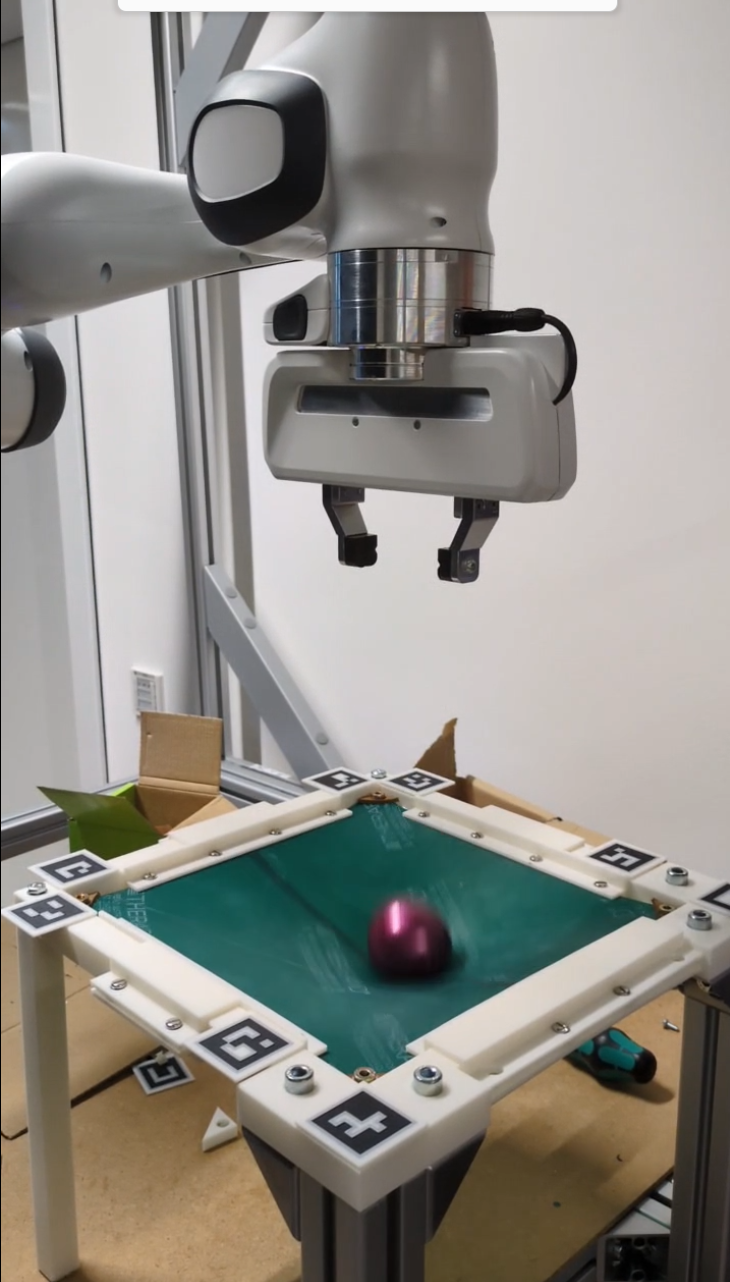
\includegraphics[width=\textwidth, trim={0 30mm 0 100mm}, clip]{figures/qualitative_realworld_data/03.png}      
%   \end{minipage}\hfill
%   \begin{minipage}{0.44\textwidth}
%     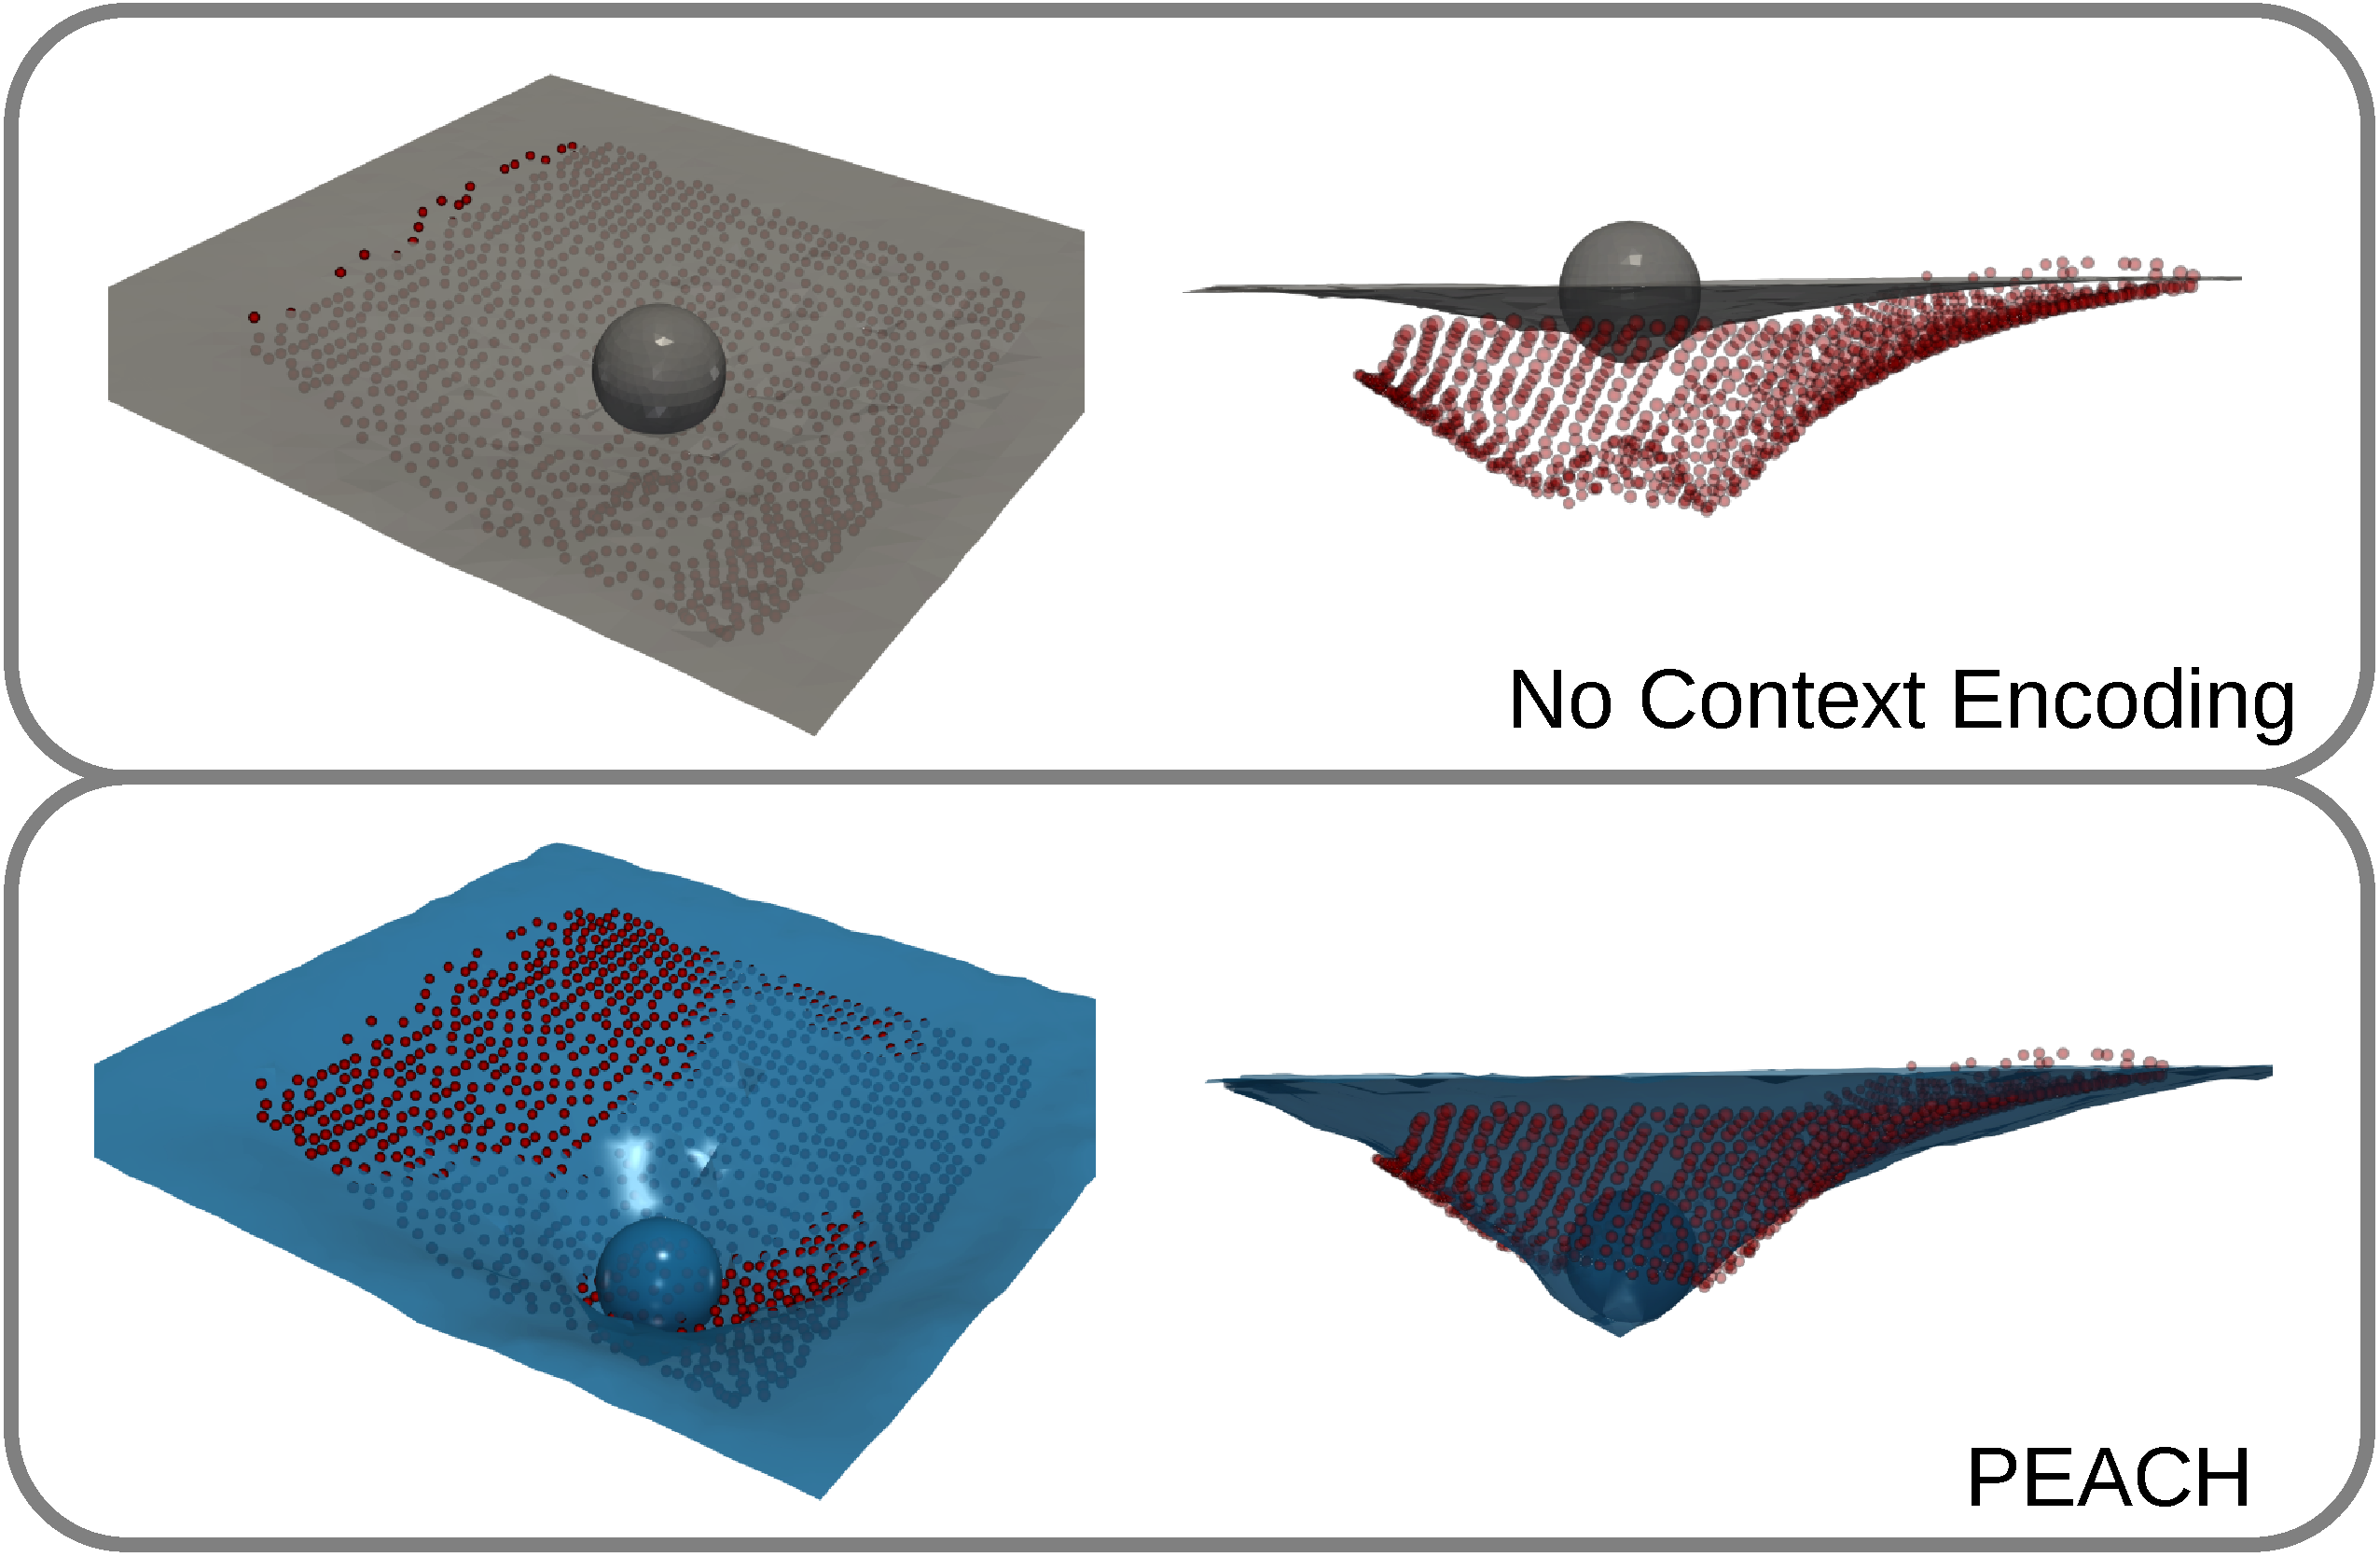
\includegraphics[width=\textwidth]{figures/qualitative_realworld_data/real_world_qualitative2.pdf}    
%   \end{minipage}
%   \begin{minipage}{0.33\textwidth}
%         \centering
%         \scalebox{0.73}{% This file was created with matplot2tikz v0.5.1.
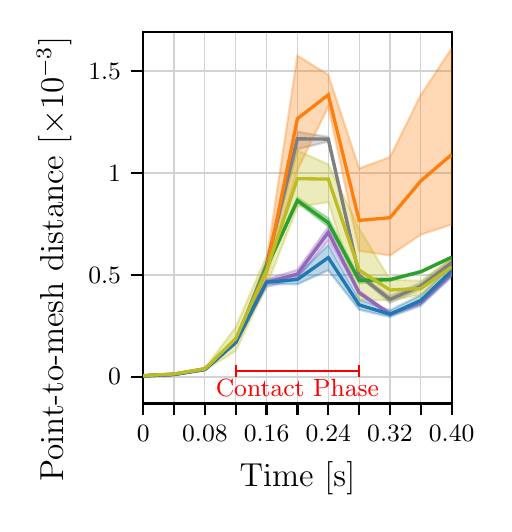
\begin{tikzpicture}

\definecolor{darkgray}{RGB}{169,169,169}
\definecolor{darkorange25512714}{RGB}{255,127,14}
\definecolor{darkslategray38}{RGB}{38,38,38}
\definecolor{forestgreen4416044}{RGB}{44,160,44}
\definecolor{goldenrod18818934}{RGB}{188,189,34}
\definecolor{gray127}{RGB}{127,127,127}
\definecolor{lightgray204}{RGB}{204,204,204}
\definecolor{steelblue31119180}{RGB}{31,119,180}
\definecolor{mediumpurple148103189}{RGB}{148,103,189}

\begin{axis}[
    line width=0.8pt,
    axis line style={black},
    height=6.3cm,
    width=5.5cm,
    legend cell align={left},
    legend style={
      fill opacity=0.8,
      draw opacity=1,
      text opacity=1,
      at={(0.03,0.97)},
      anchor=north west,
      draw=lightgray204
    },
    % legend to name=distlegend,
    % legend columns=4,
    % legend cell align={left},
    % legend style={
    %   draw=lightgray204,
    %   fill=white,
    %   fill opacity=0.9,
    %   text opacity=1,
    %   font=\scriptsize,
    %   /tikz/every even column/.append style={column sep=5pt}
    % },
    tick align=outside,
    xlabel={Time [s]},
    xlabel style={font=\large, color=black},
    ylabel={Point-to-mesh distance [$\times10^{-3}$]},
    scaled y ticks=false,
    yticklabel={
      \pgfmathparse{\tick*1000}
      \pgfmathprintnumber[fixed,precision=1]{\pgfmathresult}
    },
    ylabel style={font=\large, color=black, xshift=-15pt,yshift=-1pt},
    tick label style={font=\small, color=black},
    xmajorgrids,
    xmajorticks=true,
    xtick pos=bottom,
    xmin=0, xmax=10,
    xtick={0,1,2,3,4,5,6,7,8,9,10},
    xticklabels={0, , 0.08, , 0.16, , 0.24, , 0.32, , 0.40},
    xtick style={color=black, line width=0.8pt},
    x grid style={lightgray!70},
    ymajorgrids,
    ymin=-0.00013, ymax=0.00169170054904424,
    ytick pos=left,
    ytick style={color=black, line width=0.8pt},
    y grid style={lightgray!70},
    mark size=1.5pt,
]
\path [draw=gray127, fill=gray127, opacity=0.3]
(axis cs:0,8.11894773903532e-06)
--(axis cs:0,5.12359331139578e-06)
--(axis cs:1,1.24465407043317e-05)
--(axis cs:2,3.70390871940742e-05)
--(axis cs:3,0.000170088983293226)
--(axis cs:4,0.000538726298991605)
--(axis cs:5,0.00111711371160709)
--(axis cs:6,0.0011539952494968)
--(axis cs:7,0.000493944165682478)
--(axis cs:8,0.000363235438599077)
--(axis cs:9,0.000430066142989745)
--(axis cs:10,0.000541865832110489)
--(axis cs:10,0.000579374625937817)
--(axis cs:10,0.000579374625937817)
--(axis cs:9,0.000462110629396193)
--(axis cs:8,0.000397154613974635)
--(axis cs:7,0.000502686903510039)
--(axis cs:6,0.00117717037701368)
--(axis cs:5,0.00120230794382223)
--(axis cs:4,0.000562686173348084)
--(axis cs:3,0.000175566404236633)
--(axis cs:2,3.94724731199858e-05)
--(axis cs:1,1.48924968993924e-05)
--(axis cs:0,8.11894773903532e-06)
--cycle;

\path [draw=darkorange25512714, fill=darkorange25512714, opacity=0.3]
(axis cs:0,5.40829057285919e-06)
--(axis cs:0,5.12708819030649e-06)
--(axis cs:1,1.26935416273e-05)
--(axis cs:2,3.87968943675787e-05)
--(axis cs:3,0.000167262485056199)
--(axis cs:4,0.00048637886969118)
--(axis cs:5,0.00101407638474484)
--(axis cs:6,0.00132488404211472)
--(axis cs:7,0.000618741954658617)
--(axis cs:8,0.00059531467425586)
--(axis cs:9,0.000698201175291615)
--(axis cs:10,0.000747446074487471)
--(axis cs:10,0.00161138177505563)
--(axis cs:10,0.00161138177505563)
--(axis cs:9,0.0013830343025802)
--(axis cs:8,0.00107759078622621)
--(axis cs:7,0.0010224056098923)
--(axis cs:6,0.00148174712423497)
--(axis cs:5,0.00157530098460938)
--(axis cs:4,0.000571288045344374)
--(axis cs:3,0.000169920463772542)
--(axis cs:2,4.35155251142305e-05)
--(axis cs:1,1.37517620123617e-05)
--(axis cs:0,5.40829057285919e-06)
--cycle;

\path [draw=forestgreen4416044, fill=forestgreen4416044, opacity=0.3]
(axis cs:0,5.02886968320126e-06)
--(axis cs:0,5.00629528346508e-06)
--(axis cs:1,1.22442673364276e-05)
--(axis cs:2,3.64980695599115e-05)
--(axis cs:3,0.000170152035236697)
--(axis cs:4,0.000532057652440017)
--(axis cs:5,0.000854251318701245)
--(axis cs:6,0.000737646454490459)
--(axis cs:7,0.00045989315263796)
--(axis cs:8,0.000471600066430256)
--(axis cs:9,0.000512676674770773)
--(axis cs:10,0.000583336630952544)
--(axis cs:10,0.00059101728056703)
--(axis cs:10,0.00059101728056703)
--(axis cs:9,0.000519406470630202)
--(axis cs:8,0.000481395700517169)
--(axis cs:7,0.00048684069643059)
--(axis cs:6,0.000778906577484122)
--(axis cs:5,0.000879407519557844)
--(axis cs:4,0.000544052049326638)
--(axis cs:3,0.000173569310650237)
--(axis cs:2,3.67153696726064e-05)
--(axis cs:1,1.23036071607885e-05)
--(axis cs:0,5.02886968320126e-06)
--cycle;

\path [draw=mediumpurple148103189, fill=mediumpurple148103189, opacity=0.3]
(axis cs:0,5.71805394145031e-06)
--(axis cs:0,5.01869094364338e-06)
--(axis cs:1,1.22791177000181e-05)
--(axis cs:2,3.65818932192497e-05)
--(axis cs:3,0.000167055152474461)
--(axis cs:4,0.000440917325113333)
--(axis cs:5,0.000484037372771127)
--(axis cs:6,0.00066896209913466)
--(axis cs:7,0.000405467094214259)
--(axis cs:8,0.000302540388506713)
--(axis cs:9,0.000360184482306067)
--(axis cs:10,0.000494188704960834)
--(axis cs:10,0.000520897211245028)
--(axis cs:10,0.000520897211245028)
--(axis cs:9,0.000368405658828124)
--(axis cs:8,0.000314538892644123)
--(axis cs:7,0.000422770715022125)
--(axis cs:6,0.000736019156793191)
--(axis cs:5,0.000525294678845967)
--(axis cs:4,0.000479866894897896)
--(axis cs:3,0.000170394556655538)
--(axis cs:2,3.7254243580378e-05)
--(axis cs:1,1.29903018734012e-05)
--(axis cs:0,5.71805394145031e-06)
--cycle;

\path [draw=steelblue31119180, fill=steelblue31119180, opacity=0.3]
(axis cs:0,5.32954746347514e-06)
--(axis cs:0,5.02559393680713e-06)
--(axis cs:1,1.23061595667195e-05)
--(axis cs:2,3.64593142171543e-05)
--(axis cs:3,0.000167017648384444)
--(axis cs:4,0.000454926606626032)
--(axis cs:5,0.000454583113850049)
--(axis cs:6,0.000523227875182783)
--(axis cs:7,0.000330028291073177)
--(axis cs:8,0.00029419582178889)
--(axis cs:9,0.000349462154376852)
--(axis cs:10,0.000491633596502652)
--(axis cs:10,0.00054824294982609)
--(axis cs:10,0.00054824294982609)
--(axis cs:9,0.000401096724481249)
--(axis cs:8,0.000327221116303917)
--(axis cs:7,0.000380109390453072)
--(axis cs:6,0.000647119674776377)
--(axis cs:5,0.000497473443410854)
--(axis cs:4,0.000475108261580317)
--(axis cs:3,0.000171479885157169)
--(axis cs:2,3.71906361107221e-05)
--(axis cs:1,1.26398031545705e-05)
--(axis cs:0,5.32954746347514e-06)
--cycle;

\path [draw=goldenrod18818934, fill=goldenrod18818934, opacity=0.3]
(axis cs:0,7.55942195667103e-06)
--(axis cs:0,5.52975005234657e-06)
--(axis cs:1,1.28374976397936e-05)
--(axis cs:2,3.3174264311242e-05)
--(axis cs:3,0.000127611329533011)
--(axis cs:4,0.00044633482837753)
--(axis cs:5,0.000834116966279907)
--(axis cs:6,0.000857031254699905)
--(axis cs:7,0.000378076702199905)
--(axis cs:8,0.000375544254748092)
--(axis cs:9,0.000402517683296537)
--(axis cs:10,0.000496598869322043)
--(axis cs:10,0.00058259550252842)
--(axis cs:10,0.00058259550252842)
--(axis cs:9,0.000471571105963449)
--(axis cs:8,0.000477151526465605)
--(axis cs:7,0.000728169816311493)
--(axis cs:6,0.0010427770119486)
--(axis cs:5,0.00110999800966965)
--(axis cs:4,0.000593933843456398)
--(axis cs:3,0.000244060702209481)
--(axis cs:2,4.2721270048105e-05)
--(axis cs:1,1.77087158789391e-05)
--(axis cs:0,7.55942195667103e-06)
--cycle;

\addplot [very thick, gray127, mark=none, forget plot]
table {%
0 6.16846661046111e-06
1 1.33566141312258e-05
2 3.79323264291998e-05
3 0.000172875483426651
4 0.000550706236169845
5 0.00116767553210593
6 0.00116614555628075
7 0.000498315534596259
8 0.000380195026286856
9 0.000446161982363265
10 0.00056057571105157
};
\addplot [very thick, darkorange25512714, mark=none, forget plot]
table {%
0 5.25982570195538e-06
1 1.32226518198308e-05
2 4.09810629054164e-05
3 0.000168443404438676
4 0.000525215963987193
5 0.00126655838633724
6 0.00138342683052542
7 0.000767640316489633
8 0.000780909799859728
9 0.00096147732127065
10 0.00109070352106755
};
\addplot [very thick, forestgreen4416044, mark=none, forget plot]
table {%
0 5.01956598668585e-06
1 1.2269513994454e-05
2 3.66266437509921e-05
3 0.000171860672943467
4 0.000536364111319472
5 0.000864933194968671
6 0.000756467673586485
7 0.000473366924534275
8 0.000477138728074351
9 0.000516041572700487
10 0.000587167208759638
};
\addplot [very thick, mediumpurple148103189, mark=none, forget plot]
table {%
0 5.35674467698755e-06
1 1.26106139231297e-05
2 3.68227403703258e-05
3 0.000169110989764931
4 0.000464556738356805
5 0.000504666025808547
6 0.000708642764411707
7 0.000413382586743865
8 0.000308661070916969
9 0.000364295070567096
10 0.000507542958102931
};
\addplot [very thick, steelblue31119180, mark=none, forget plot]
table {%
0 5.16803246910058e-06
1 1.24482370745227e-05
2 3.68488107579878e-05
3 0.000169248766770806
4 0.000465017434103174
5 0.0004779231458906
6 0.000585161942171908
7 0.000353386584361033
8 0.000307302393166537
9 0.000375522828585417
10 0.000519938273164371
};

\addplot [very thick, goldenrod18818934, mark=none, forget plot]
table {%
0 6.35538139363234e-06
1 1.47364074132383e-05
2 3.90641958421156e-05
3 0.000188316963522084
4 0.000524306058375714
5 0.00097205748797478
6 0.000970418218125815
7 0.000524069131924989
8 0.000426347890606849
9 0.000434198304646998
10 0.000539597185925231
};

\draw [red, thick] (axis cs:3, 0.00003) -- (axis cs:7, 0.00003);
\draw [red, thick] (axis cs:3, -0.0000) -- (axis cs:3,  0.00006);
\draw [red, thick] (axis cs:7, -0.0000) -- (axis cs:7,  0.00006);
\node [red, font=\small] at (axis cs:5, -0.000055) {Contact Phase};
\end{axis}

\end{tikzpicture}
}\\
%         % {\footnotesize\texttt{Trampoline (Real-world)}}
%     \end{minipage}
%     \hfill
% \caption{Real-world trampoline experiment. \textbf{Left:} Physical setup with a ball interacting with a latex sheet. \textbf{Center:} Qualitative comparison at $t=0.2\,\text{s}$ (maximal sheet elongation) between a model without context encoding and PEACH. The red point cloud shows the ground truth observations; note that the very bottom of the sheet is occluded by the ball and thus absent from the point cloud. \textbf{Right:} Point-to-mesh distance aggregated over all real-world trials, plotted over time, with ball-sheet contact occurring between $t=0.12\,\text{s}$ and $t=0.28\,\text{s}$.}
%   \label{fig:qualitative_realworld}
% \end{figure}

\begin{figure}[t]
  \centering

\makebox[\textwidth][l]{%
\scalebox{1.01}{
  \hspace*{0.015\textwidth}%
  \begin{minipage}[t]{0.25\textwidth}
    \vspace{2pt}
    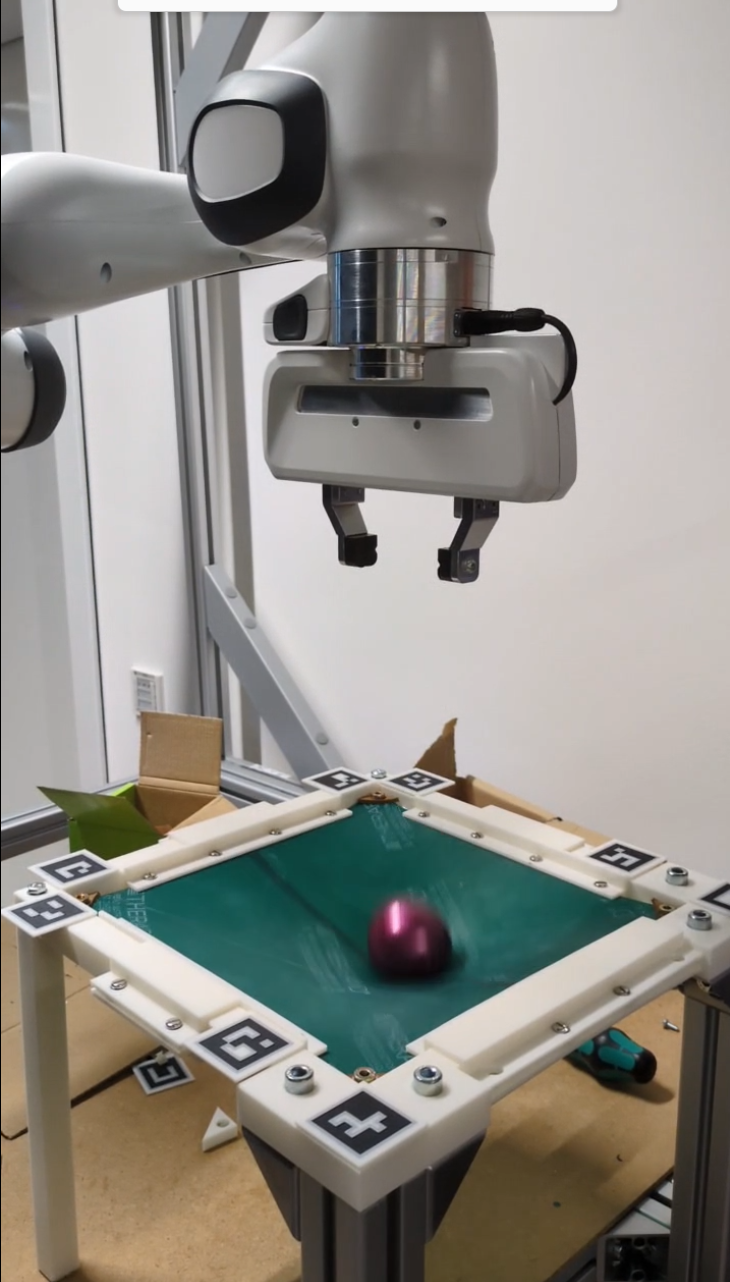
\includegraphics[
      width=\textwidth,
      trim={0 30mm 0 100mm},
      clip
    ]{figures/qualitative_realworld_data/03.png}      
  \end{minipage}\hspace{0.030\textwidth}%
  \begin{minipage}[t]{0.68\textwidth}
    \vspace{0pt}

    % Legend next to the left image, not above the whole figure

    % \begin{tikzpicture}
%     \tikzstyle{every node}=[font=\scriptsize]
%     \definecolor{tabblue}{RGB}{31, 119, 180}
\definecolor{taborange}{RGB}{255, 127, 14}
\definecolor{tabgreen}{RGB}{44, 160, 44}
\definecolor{tabred}{RGB}{214, 39, 40}
\definecolor{tabpurple}{RGB}{148, 103, 189}
\definecolor{tabbrown}{RGB}{140, 86, 75}
\definecolor{tabpink}{RGB}{227, 119, 194}
\definecolor{tabgray}{RGB}{127, 127, 127}
\definecolor{tabolive}{RGB}{188, 189, 34}
\definecolor{tabcyan}{RGB}{23, 190, 207}
\definecolor{ForestGreen}{RGB}{34, 139, 34}
%     \begin{axis}[%
%     hide axis,
%     xmin=10,
%     xmax=50,
%     ymin=0,
%     ymax=0.1,
%     legend style={
%         draw=white!15!black,
%         legend cell align=left,
%         legend columns=3,
%         legend style={
%             draw=none,
%             column sep=1ex,
%             line width=1pt,
%         }
%     },
%     ]

%     \addlegendimage{
%         line legend,
%         tabblue,
%         thick,
%         mark=square*,
%         mark options={line width=1.5pt, rotate=45}
%     }
%     \addlegendentry{\textbf{PEACH Encoder} (Ours)}
%     \addlegendimage{line legend, tabgreen, thick, mark=triangle*, mark options={line width=1.5pt, rotate=0}}
%     \addlegendentry{GNN Encoder}
%     \addlegendimage{
%         line legend,
%         taborange,
%         thick,
%         mark=square*,
%         mark options={line width=1.5pt, rotate=0}
%     }
%     \addlegendentry{PSTNet Encoder}
%     % New Line
%     % \addlegendimage{empty legend}
%     % \addlegendentry{}

%     \addlegendimage{line legend, tabolive, thick, mark=x, mark size=3pt, mark options={line width=1pt}}
%     \addlegendentry{Oracle Encoder}
%     \addlegendimage{line legend, tabcyan, thick, mark=+, mark size=2.5pt, mark options={line width=2pt}}
%     \addlegendentry{MaNGO Mesh Encoder}
%     \addlegendimage{line legend, tabgray, thick, mark=*}
%     \addlegendentry{No Context Encoder}    
%     \end{axis}
% \end{tikzpicture}

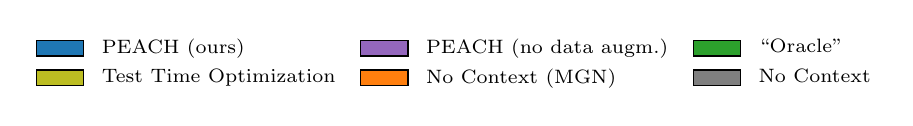
\begin{tikzpicture}
    \tikzstyle{every node}=[font=\scriptsize]
    \definecolor{tabblue}{RGB}{31, 119, 180}
\definecolor{taborange}{RGB}{255, 127, 14}
\definecolor{tabgreen}{RGB}{44, 160, 44}
\definecolor{tabred}{RGB}{214, 39, 40}
\definecolor{tabpurple}{RGB}{148, 103, 189}
\definecolor{tabbrown}{RGB}{140, 86, 75}
\definecolor{tabpink}{RGB}{227, 119, 194}
\definecolor{tabgray}{RGB}{127, 127, 127}
\definecolor{tabolive}{RGB}{188, 189, 34}
\definecolor{tabcyan}{RGB}{23, 190, 207}
\definecolor{ForestGreen}{RGB}{34, 139, 34}

    \begin{axis}[%
        hide axis,
        xmin=10,
        xmax=50,
        ymin=0,
        ymax=0.1,
        legend style={
            draw=none,
            legend cell align=left,
            legend columns=3,
            /tikz/every odd column/.append style={column sep=1ex},
            /tikz/every even column/.append style={column sep=1.6ex},
        }
    ]

    % --- Bar-style legend entries ---
    \addlegendimage{area legend, fill=tabblue}
    \addlegendentry{PEACH (ours)}

    \addlegendimage{area legend, fill=tabpurple}
    \addlegendentry{PEACH (no data augm.)}

    \addlegendimage{area legend, fill=tabgreen}
    \addlegendentry{``Oracle''}


    \addlegendimage{area legend, fill=tabolive}
    \addlegendentry{Test Time Optimization}

    
    \addlegendimage{area legend, fill=taborange}
    \addlegendentry{No Context (MGN)}

    \addlegendimage{area legend, fill=tabgray}
    \addlegendentry{No Context}
    \end{axis}
\end{tikzpicture}\\[-7mm]

    \hspace{0.000\textwidth}
    \begin{minipage}[t]{0.57\textwidth}
      \vspace{0pt}
      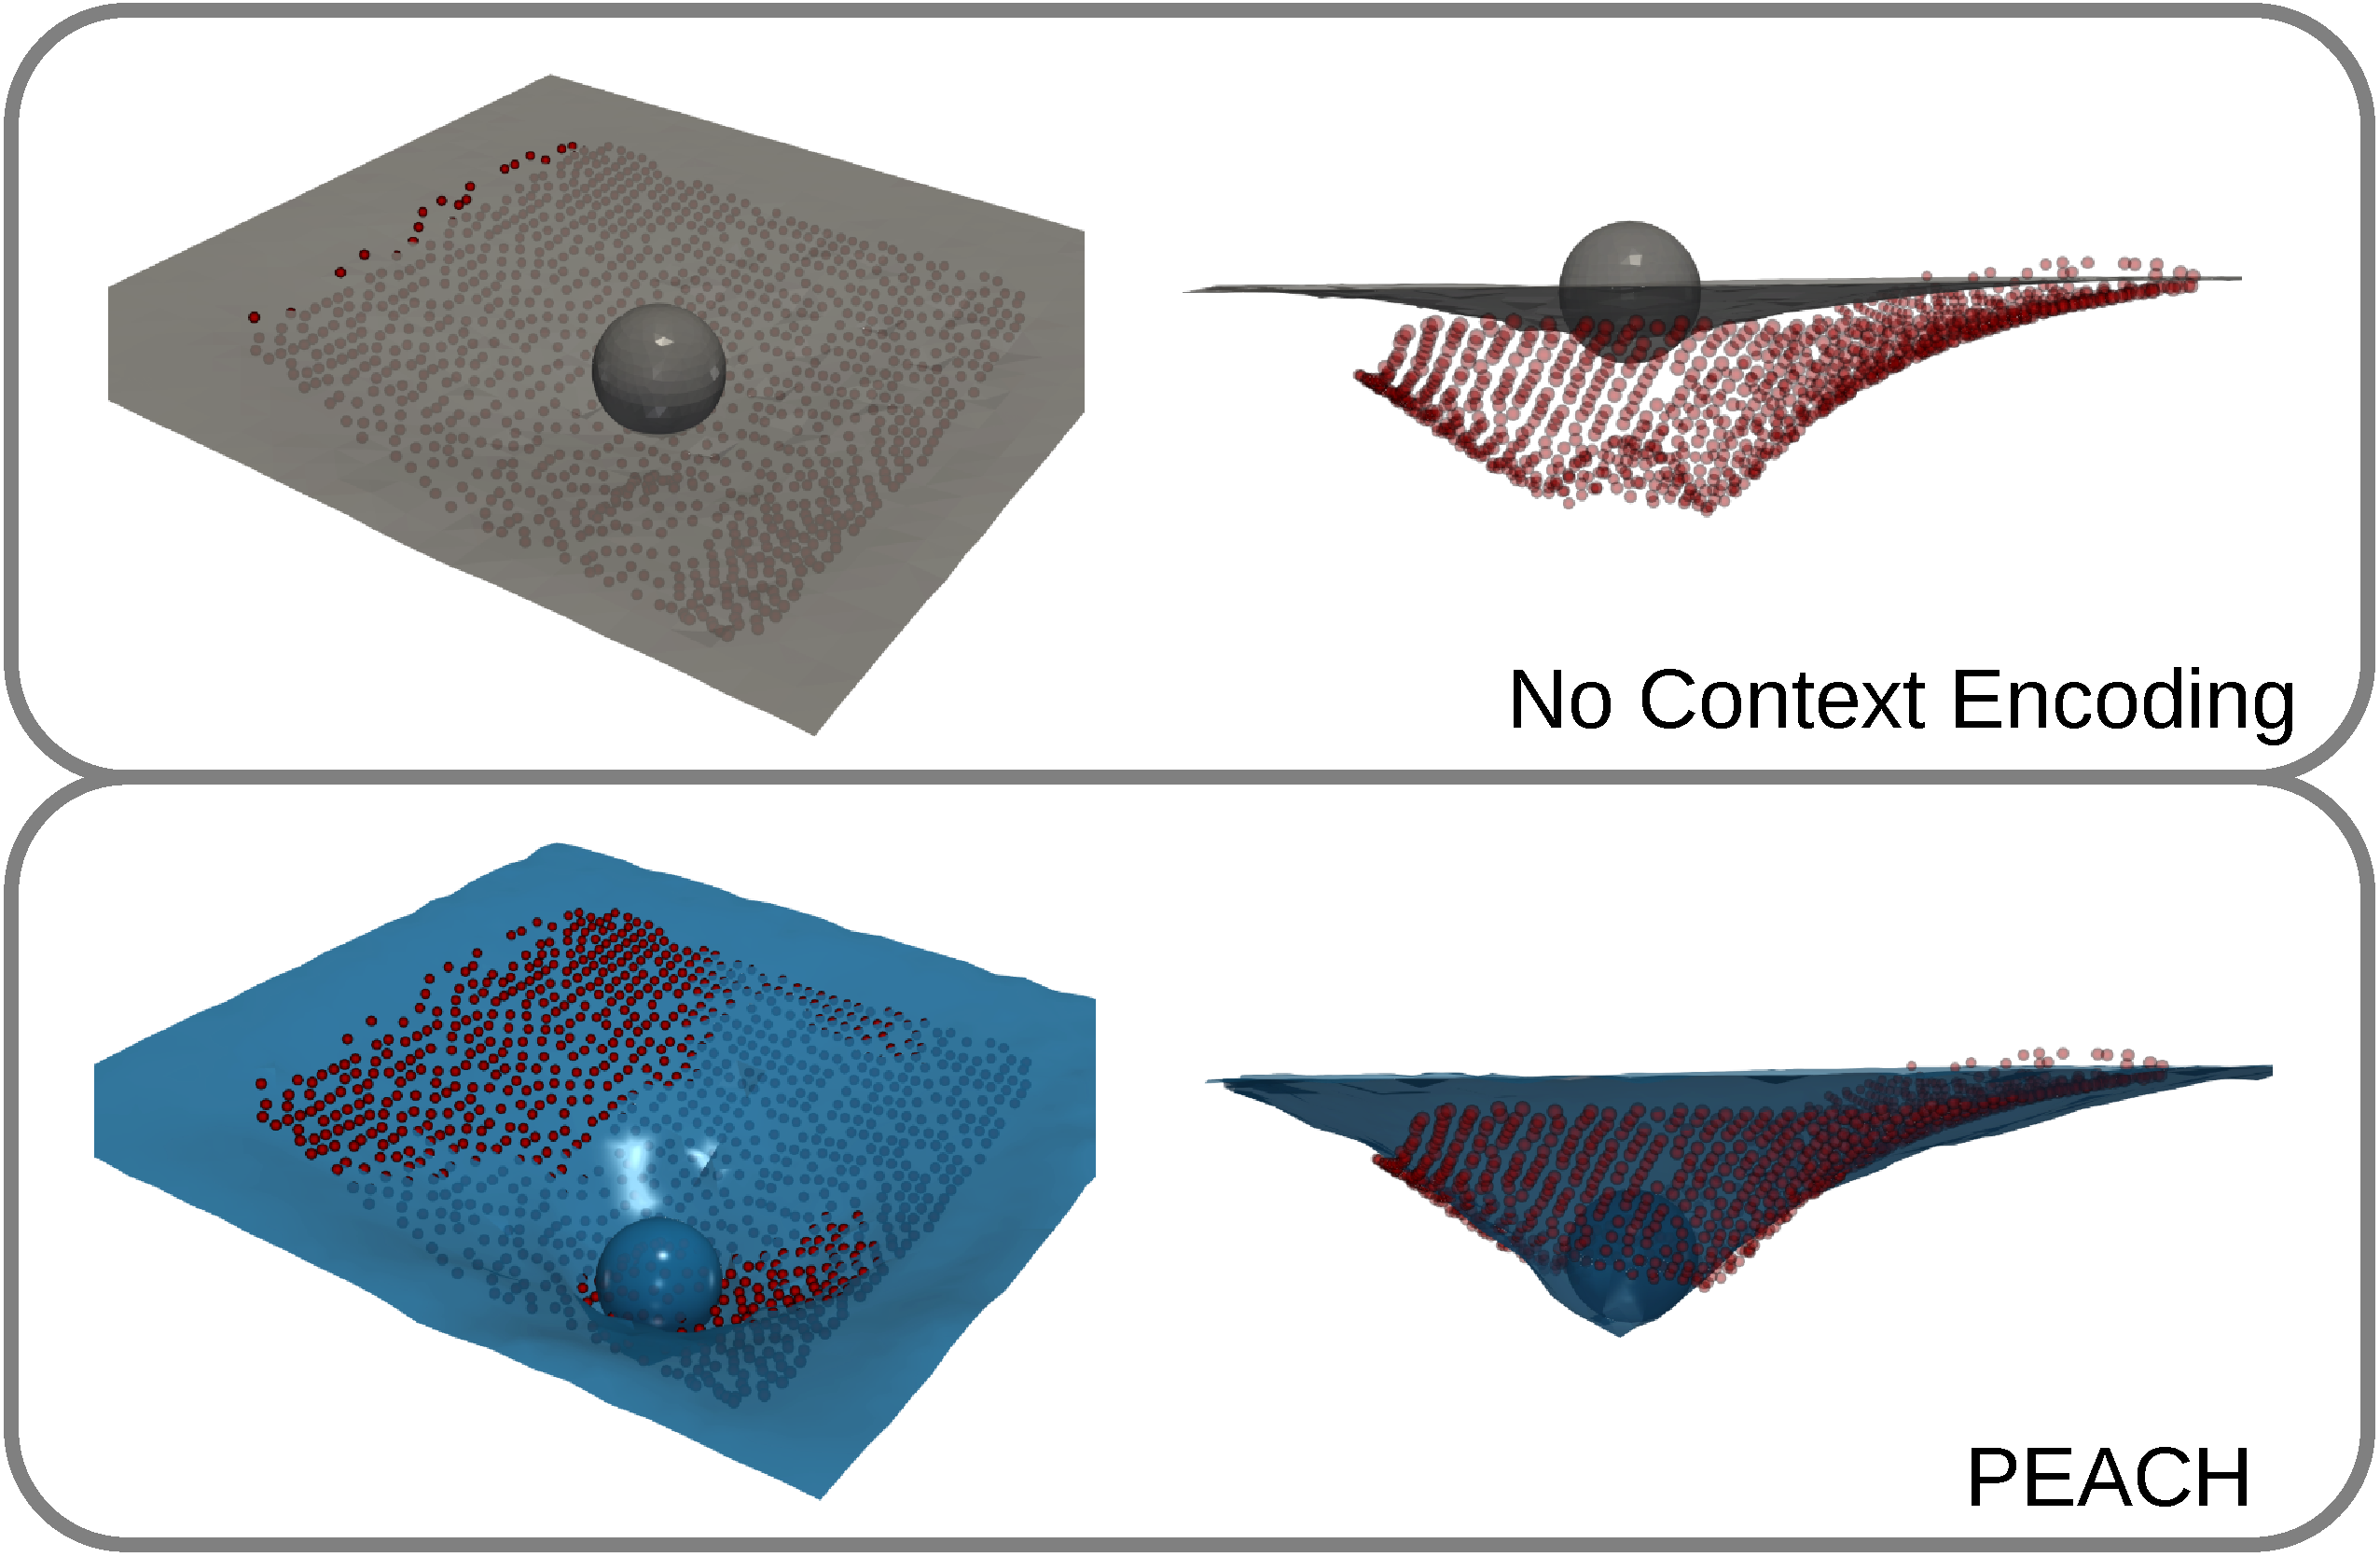
\includegraphics[
        width=\textwidth
      ]{figures/qualitative_realworld_data/real_world_qualitative2.pdf}
    \end{minipage}\hspace{0.025\textwidth}%
      \hspace{-0pt}
    \begin{minipage}[t]{0.30\textwidth}
      \vspace{0pt}   % was -10pt — now pushes the plot down instead of up
      \centering
      \scalebox{0.60}{%
        % This file was created with matplot2tikz v0.5.1.
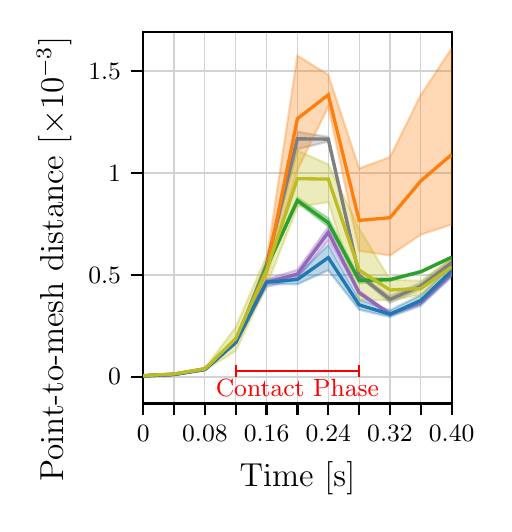
\begin{tikzpicture}

\definecolor{darkgray}{RGB}{169,169,169}
\definecolor{darkorange25512714}{RGB}{255,127,14}
\definecolor{darkslategray38}{RGB}{38,38,38}
\definecolor{forestgreen4416044}{RGB}{44,160,44}
\definecolor{goldenrod18818934}{RGB}{188,189,34}
\definecolor{gray127}{RGB}{127,127,127}
\definecolor{lightgray204}{RGB}{204,204,204}
\definecolor{steelblue31119180}{RGB}{31,119,180}
\definecolor{mediumpurple148103189}{RGB}{148,103,189}

\begin{axis}[
    line width=0.8pt,
    axis line style={black},
    height=6.3cm,
    width=5.5cm,
    legend cell align={left},
    legend style={
      fill opacity=0.8,
      draw opacity=1,
      text opacity=1,
      at={(0.03,0.97)},
      anchor=north west,
      draw=lightgray204
    },
    % legend to name=distlegend,
    % legend columns=4,
    % legend cell align={left},
    % legend style={
    %   draw=lightgray204,
    %   fill=white,
    %   fill opacity=0.9,
    %   text opacity=1,
    %   font=\scriptsize,
    %   /tikz/every even column/.append style={column sep=5pt}
    % },
    tick align=outside,
    xlabel={Time [s]},
    xlabel style={font=\large, color=black},
    ylabel={Point-to-mesh distance [$\times10^{-3}$]},
    scaled y ticks=false,
    yticklabel={
      \pgfmathparse{\tick*1000}
      \pgfmathprintnumber[fixed,precision=1]{\pgfmathresult}
    },
    ylabel style={font=\large, color=black, xshift=-15pt,yshift=-1pt},
    tick label style={font=\small, color=black},
    xmajorgrids,
    xmajorticks=true,
    xtick pos=bottom,
    xmin=0, xmax=10,
    xtick={0,1,2,3,4,5,6,7,8,9,10},
    xticklabels={0, , 0.08, , 0.16, , 0.24, , 0.32, , 0.40},
    xtick style={color=black, line width=0.8pt},
    x grid style={lightgray!70},
    ymajorgrids,
    ymin=-0.00013, ymax=0.00169170054904424,
    ytick pos=left,
    ytick style={color=black, line width=0.8pt},
    y grid style={lightgray!70},
    mark size=1.5pt,
]
\path [draw=gray127, fill=gray127, opacity=0.3]
(axis cs:0,8.11894773903532e-06)
--(axis cs:0,5.12359331139578e-06)
--(axis cs:1,1.24465407043317e-05)
--(axis cs:2,3.70390871940742e-05)
--(axis cs:3,0.000170088983293226)
--(axis cs:4,0.000538726298991605)
--(axis cs:5,0.00111711371160709)
--(axis cs:6,0.0011539952494968)
--(axis cs:7,0.000493944165682478)
--(axis cs:8,0.000363235438599077)
--(axis cs:9,0.000430066142989745)
--(axis cs:10,0.000541865832110489)
--(axis cs:10,0.000579374625937817)
--(axis cs:10,0.000579374625937817)
--(axis cs:9,0.000462110629396193)
--(axis cs:8,0.000397154613974635)
--(axis cs:7,0.000502686903510039)
--(axis cs:6,0.00117717037701368)
--(axis cs:5,0.00120230794382223)
--(axis cs:4,0.000562686173348084)
--(axis cs:3,0.000175566404236633)
--(axis cs:2,3.94724731199858e-05)
--(axis cs:1,1.48924968993924e-05)
--(axis cs:0,8.11894773903532e-06)
--cycle;

\path [draw=darkorange25512714, fill=darkorange25512714, opacity=0.3]
(axis cs:0,5.40829057285919e-06)
--(axis cs:0,5.12708819030649e-06)
--(axis cs:1,1.26935416273e-05)
--(axis cs:2,3.87968943675787e-05)
--(axis cs:3,0.000167262485056199)
--(axis cs:4,0.00048637886969118)
--(axis cs:5,0.00101407638474484)
--(axis cs:6,0.00132488404211472)
--(axis cs:7,0.000618741954658617)
--(axis cs:8,0.00059531467425586)
--(axis cs:9,0.000698201175291615)
--(axis cs:10,0.000747446074487471)
--(axis cs:10,0.00161138177505563)
--(axis cs:10,0.00161138177505563)
--(axis cs:9,0.0013830343025802)
--(axis cs:8,0.00107759078622621)
--(axis cs:7,0.0010224056098923)
--(axis cs:6,0.00148174712423497)
--(axis cs:5,0.00157530098460938)
--(axis cs:4,0.000571288045344374)
--(axis cs:3,0.000169920463772542)
--(axis cs:2,4.35155251142305e-05)
--(axis cs:1,1.37517620123617e-05)
--(axis cs:0,5.40829057285919e-06)
--cycle;

\path [draw=forestgreen4416044, fill=forestgreen4416044, opacity=0.3]
(axis cs:0,5.02886968320126e-06)
--(axis cs:0,5.00629528346508e-06)
--(axis cs:1,1.22442673364276e-05)
--(axis cs:2,3.64980695599115e-05)
--(axis cs:3,0.000170152035236697)
--(axis cs:4,0.000532057652440017)
--(axis cs:5,0.000854251318701245)
--(axis cs:6,0.000737646454490459)
--(axis cs:7,0.00045989315263796)
--(axis cs:8,0.000471600066430256)
--(axis cs:9,0.000512676674770773)
--(axis cs:10,0.000583336630952544)
--(axis cs:10,0.00059101728056703)
--(axis cs:10,0.00059101728056703)
--(axis cs:9,0.000519406470630202)
--(axis cs:8,0.000481395700517169)
--(axis cs:7,0.00048684069643059)
--(axis cs:6,0.000778906577484122)
--(axis cs:5,0.000879407519557844)
--(axis cs:4,0.000544052049326638)
--(axis cs:3,0.000173569310650237)
--(axis cs:2,3.67153696726064e-05)
--(axis cs:1,1.23036071607885e-05)
--(axis cs:0,5.02886968320126e-06)
--cycle;

\path [draw=mediumpurple148103189, fill=mediumpurple148103189, opacity=0.3]
(axis cs:0,5.71805394145031e-06)
--(axis cs:0,5.01869094364338e-06)
--(axis cs:1,1.22791177000181e-05)
--(axis cs:2,3.65818932192497e-05)
--(axis cs:3,0.000167055152474461)
--(axis cs:4,0.000440917325113333)
--(axis cs:5,0.000484037372771127)
--(axis cs:6,0.00066896209913466)
--(axis cs:7,0.000405467094214259)
--(axis cs:8,0.000302540388506713)
--(axis cs:9,0.000360184482306067)
--(axis cs:10,0.000494188704960834)
--(axis cs:10,0.000520897211245028)
--(axis cs:10,0.000520897211245028)
--(axis cs:9,0.000368405658828124)
--(axis cs:8,0.000314538892644123)
--(axis cs:7,0.000422770715022125)
--(axis cs:6,0.000736019156793191)
--(axis cs:5,0.000525294678845967)
--(axis cs:4,0.000479866894897896)
--(axis cs:3,0.000170394556655538)
--(axis cs:2,3.7254243580378e-05)
--(axis cs:1,1.29903018734012e-05)
--(axis cs:0,5.71805394145031e-06)
--cycle;

\path [draw=steelblue31119180, fill=steelblue31119180, opacity=0.3]
(axis cs:0,5.32954746347514e-06)
--(axis cs:0,5.02559393680713e-06)
--(axis cs:1,1.23061595667195e-05)
--(axis cs:2,3.64593142171543e-05)
--(axis cs:3,0.000167017648384444)
--(axis cs:4,0.000454926606626032)
--(axis cs:5,0.000454583113850049)
--(axis cs:6,0.000523227875182783)
--(axis cs:7,0.000330028291073177)
--(axis cs:8,0.00029419582178889)
--(axis cs:9,0.000349462154376852)
--(axis cs:10,0.000491633596502652)
--(axis cs:10,0.00054824294982609)
--(axis cs:10,0.00054824294982609)
--(axis cs:9,0.000401096724481249)
--(axis cs:8,0.000327221116303917)
--(axis cs:7,0.000380109390453072)
--(axis cs:6,0.000647119674776377)
--(axis cs:5,0.000497473443410854)
--(axis cs:4,0.000475108261580317)
--(axis cs:3,0.000171479885157169)
--(axis cs:2,3.71906361107221e-05)
--(axis cs:1,1.26398031545705e-05)
--(axis cs:0,5.32954746347514e-06)
--cycle;

\path [draw=goldenrod18818934, fill=goldenrod18818934, opacity=0.3]
(axis cs:0,7.55942195667103e-06)
--(axis cs:0,5.52975005234657e-06)
--(axis cs:1,1.28374976397936e-05)
--(axis cs:2,3.3174264311242e-05)
--(axis cs:3,0.000127611329533011)
--(axis cs:4,0.00044633482837753)
--(axis cs:5,0.000834116966279907)
--(axis cs:6,0.000857031254699905)
--(axis cs:7,0.000378076702199905)
--(axis cs:8,0.000375544254748092)
--(axis cs:9,0.000402517683296537)
--(axis cs:10,0.000496598869322043)
--(axis cs:10,0.00058259550252842)
--(axis cs:10,0.00058259550252842)
--(axis cs:9,0.000471571105963449)
--(axis cs:8,0.000477151526465605)
--(axis cs:7,0.000728169816311493)
--(axis cs:6,0.0010427770119486)
--(axis cs:5,0.00110999800966965)
--(axis cs:4,0.000593933843456398)
--(axis cs:3,0.000244060702209481)
--(axis cs:2,4.2721270048105e-05)
--(axis cs:1,1.77087158789391e-05)
--(axis cs:0,7.55942195667103e-06)
--cycle;

\addplot [very thick, gray127, mark=none, forget plot]
table {%
0 6.16846661046111e-06
1 1.33566141312258e-05
2 3.79323264291998e-05
3 0.000172875483426651
4 0.000550706236169845
5 0.00116767553210593
6 0.00116614555628075
7 0.000498315534596259
8 0.000380195026286856
9 0.000446161982363265
10 0.00056057571105157
};
\addplot [very thick, darkorange25512714, mark=none, forget plot]
table {%
0 5.25982570195538e-06
1 1.32226518198308e-05
2 4.09810629054164e-05
3 0.000168443404438676
4 0.000525215963987193
5 0.00126655838633724
6 0.00138342683052542
7 0.000767640316489633
8 0.000780909799859728
9 0.00096147732127065
10 0.00109070352106755
};
\addplot [very thick, forestgreen4416044, mark=none, forget plot]
table {%
0 5.01956598668585e-06
1 1.2269513994454e-05
2 3.66266437509921e-05
3 0.000171860672943467
4 0.000536364111319472
5 0.000864933194968671
6 0.000756467673586485
7 0.000473366924534275
8 0.000477138728074351
9 0.000516041572700487
10 0.000587167208759638
};
\addplot [very thick, mediumpurple148103189, mark=none, forget plot]
table {%
0 5.35674467698755e-06
1 1.26106139231297e-05
2 3.68227403703258e-05
3 0.000169110989764931
4 0.000464556738356805
5 0.000504666025808547
6 0.000708642764411707
7 0.000413382586743865
8 0.000308661070916969
9 0.000364295070567096
10 0.000507542958102931
};
\addplot [very thick, steelblue31119180, mark=none, forget plot]
table {%
0 5.16803246910058e-06
1 1.24482370745227e-05
2 3.68488107579878e-05
3 0.000169248766770806
4 0.000465017434103174
5 0.0004779231458906
6 0.000585161942171908
7 0.000353386584361033
8 0.000307302393166537
9 0.000375522828585417
10 0.000519938273164371
};

\addplot [very thick, goldenrod18818934, mark=none, forget plot]
table {%
0 6.35538139363234e-06
1 1.47364074132383e-05
2 3.90641958421156e-05
3 0.000188316963522084
4 0.000524306058375714
5 0.00097205748797478
6 0.000970418218125815
7 0.000524069131924989
8 0.000426347890606849
9 0.000434198304646998
10 0.000539597185925231
};

\draw [red, thick] (axis cs:3, 0.00003) -- (axis cs:7, 0.00003);
\draw [red, thick] (axis cs:3, -0.0000) -- (axis cs:3,  0.00006);
\draw [red, thick] (axis cs:7, -0.0000) -- (axis cs:7,  0.00006);
\node [red, font=\small] at (axis cs:5, -0.000055) {Contact Phase};
\end{axis}

\end{tikzpicture}
%
      }
    \end{minipage}
  \end{minipage}%
}
}

    \caption{
        Real-world \texttt{Trampoline} scene.
        \textbf{Left:} Physical setup with a ball bouncing on a latex sheet.
        \textbf{Center:} Qualitative comparison at $t{=}0.2\,\text{s}$ (maximal sheet stretching) between \gls{peach} and a context-free simulator.
        The \textcolor{red}{red} point cloud shows the ground truth observations. The  bottom of the sheet is occluded by the ball and thus absent from the point cloud.
        \textbf{Right:} Mean point-to-mesh distance over all real-world trials, plotted over time, with ball-sheet contact occurring in $[0.12,0.28]\, \text{s}$.
    }
    \vspace{-0.4cm}
    \label{fig:qualitative_realworld}
\end{figure}

\textbf{Scenes.}
We evaluate the sim-to-real capability of \gls{peach} on a novel scene called \texttt{Trampoline} that involves dynamic motion, complex contact interactions, and deformable objects.
Additionally, we introduce the novel simulation-only dataset \texttt{Bending Beam} inspired by \citet{wurth2025diffusion}, and adopt two existing datasets, \texttt{Deforming Block} and \texttt{Sheet Deformation}~\citep{dahlinger2025mango}\footnote{Called \texttt{Deformable Plate} (\textit{easy}) and \texttt{Planar Bending}, respectively, in \citet{dahlinger2025mango}.}.
These scenes span 2D and 3D domains, and are inspired by simulation-assisted process optimization in industrial contexts.
They feature varying physical parameters such as Young's modulus (all except \texttt{Deforming Block}), Poisson's ratio (all except \texttt{Sheet Deformation}), membrane thickness, shear relaxation ratio (\texttt{Trampoline}), and relaxation time (\texttt{Bending Beam} and \texttt{Trampoline}).
Rollout length varies by scene from $25$ (\texttt{Trampoline}) to $100$ (\texttt{Bending Beam}).
Although the \texttt{Trampoline} scene has a shorter horizon, it has the most complex geometry, with roughly $10$ times more triangles than other scenes.
A visual overview of the scenes is provided in Figure~\ref{fig:task_overview}, with further details in Appendix~\ref{app:dataset}.

In simulation, we obtain per-step point clouds by ray casting from a static camera and applying \gls{fps}~\citep{ruizhongtai2017pointnet} to retain $512$ points; due to the finer geometry \texttt{Trampoline} uses $1024$ points.
To reduce the point cloud sequence length, we drop every $2$nd time step. 
In \texttt{Trampoline} and \texttt{Deforming Block}, collider points are explicitly marked.
For the real world \texttt{Trampoline} dataset, we use a robot to drop balls of varying density onto latex sheets of different thicknesses and record depth images with a ZED Mini Stereo Camera (Stereolabs).
Neither meshes nor ground truth physical parameters are known for these recordings.
For the ``\textit{Oracle}'' baseline, measurable material properties are determined experimentally  while the remaining parameters are chosen based on informed estimates from literature values.
Appendix~\ref{app:real} details the real-world data.

\textbf{Baselines.}
We compare \gls{peach} against methods using $4$ different context types, namely point cloud contexts, mesh contexts, oracle, and no context.
\textit{Oracle} methods receive the ground truth physical properties at every time step as additional node features.
\textit{No Context} methods predict trajectories solely from the initial state without additional task information.
Methods using point cloud contexts infer the task from the same context point cloud sequences as \gls{peach}.
\textit{PSTNet Encoder}~\citep{fan2021pstnet} and \textit{GNN Encoder} differ from \gls{peach} only in the encoder architecture.
\textit{PSTNet Encoder} captures local geometric evolution via space-time tubes anchored at \gls{fps}-sampled reference points, applying decoupled spatial and temporal convolutions hierarchically across the point cloud sequence.
\textit{GNN Encoder} adapts the graph network paradigm from mesh-based simulation to point cloud sequences.
It tokenizes each timestep's point cloud into local patch embeddings, constructs a spatio-temporal graph connecting tokens within and across adjacent frames, and processes it via message passing with a final readout into a trajectory-level latent code.
\textit{Test-Time Optimization} instead follows the classical system identification paradigm.
Starting from the mean training parameters, it optimizes the physical parameters of the trained \textit{Oracle} model by gradient descent through the simulator, minimizing the distance between the observed context point clouds and the predicted meshes.

\gls{mango}~\citep{dahlinger2025mango} instead computes the latent embedding using privileged mesh contexts.
Since such contexts are not readily available in real-world settings, \gls{mango} is not directly comparable to our method, but demonstrates the impact of replacing explicit mesh observations with point clouds in simulated tasks.
All baselines that predict a latent embedding also receive auxiliary supervision via ground truth physical properties.

Lastly, we study the impact of the simulator component by replacing the MaNGO simulator with the \gls{mgn} simulator~\citep{pfaff2020learning}, a mesh-based autoregressive simulator trained for one-step prediction.
We instantiate the \gls{mgn} baseline in \textit{Oracle (\gls{mgn})} and \textit{No Context (\gls{mgn})} variants.
While it is possible to integrate \gls{mgn} into the \gls{peach} framework, early experiments indicated that it was outperformed by the MaNGO simulator.
Appendix~\ref{app:methods} details all baselines.

\textbf{Training.}
We train each method end-to-end.
All in-context methods are trained using batches of $1$ to $8$ randomly sampled context trajectories to improve adaptation capability.
We repeat each experiment across $4$ random seeds using the AdamW optimizer~\citep{adamw} with a learning rate of $5.0{\times}10^{-5}$.
All methods were trained on either an A100 or H100 GPU for $2$ days, with the exception of \texttt{Bending Beam}, which converged after $1$ day.
Appendix~\ref{app:hp} lists hyperparameters, and Appendix~\ref{sec:runtime} provides parameter counts, inference runtimes, and an analysis of how the encoding time scales with context size, point count, and trajectory length.
